\documentclass[aspectratio=169]{beamer}
\useoutertheme[progressbar=frametitle]{metropolis}
\useinnertheme{metropolis}
\definecolor{nabgray}{rgb}{0.6,0.59,0.61}
\usecolortheme[named=nabgray]{structure}
\usepackage{tikz}
\usepackage[utf8]{inputenc}
\usepackage[spanish]{babel}
\usepackage{fontspec}
\setmonofont{JetBrains Mono}
\setmainfont{Roboto}
\setsansfont{Roboto}

\usepackage{smartdiagram}
\usepackage{qtree}
\usepackage{verbatim}
\usepackage{svg}
\usepackage{graphicx}
\usepackage{color}
\definecolor{lightgray}{rgb}{0.95, 0.95, 0.95}
\definecolor{darkgray}{rgb}{0.4, 0.4, 0.4}
\definecolor{ocherCode}{rgb}{1, 0.5, 0} % #FF7F00 -> rgb(239, 169, 0)
\definecolor{blueCode}{rgb}{0, 0, 0.93} % #0000EE -> rgb(0, 0, 238)
\definecolor{greenCode}{rgb}{0, 0.6, 0} % #009900 -> rgb(0, 153, 0)

\usepackage{upquote}
\usepackage{listings}
\lstset{language=java,
    otherkeywords={var,record},
	% Basic design
	backgroundcolor=\color{lightgray},
	basicstyle={\small\ttfamily},
	frame=l,
	keywordstyle=\footnotesize\color{blue},
	escapeinside={<@}{@>},
	breaklines=true,
	% Line numbers
	xleftmargin={0.75cm},
	numbers=left,
	stepnumber=1,
	firstnumber=1,
	numberfirstline=true
	% Code design
	identifierstyle=\color{black},
	keywordstyle=\color{ocherCode}\bfseries,
	ndkeywordstyle=\color{greenCode}\bfseries,
	stringstyle=\color{ocherCode}\ttfamily,
	commentstyle=\color{darkgray}\ttfamily,
	tabsize=2,
	showtabs=true,
	showspaces=false,
	showstringspaces=false,
	extendedchars=true,
	breaklines=true
}

\lstdefinelanguage{bash}{
    basicstyle=\ttfamily,
    showstringspaces=false,
    commentstyle=\color{red},
    keywordstyle=\color{blue},
    numbers=right,
    xleftmargin={0.25cm}
}

\usebackgroundtemplate
{
	
\includegraphics[width=\paperwidth]{Images/fondo}%
}


\title{Bootstraping real world Jakarta EE/MicroProfile microservices with Maven Archetypes}
\author{Víctor Orozco - @tuxtor}
\institute{Software architect}
\date{\today}

\begin{document}

{
    \usebackgroundtemplate{
\includegraphics[width=\paperwidth]{Images/portada}}
    \setbeamercolor{frametitle}{fg=red}
    \usebeamercolor[fg]{normal text}
    \frame{\titlepage}
}


%\begin{frame}{Microservice}
%What is a microservice anyway?

%\begin{itemize}
%\item Processes that communicate over a network to fulfil a goal using technology-agnostic protocols such as HTTP
%\item Organized around business capabilities.
%\item \textbf{Implemented using different programming languages, databases, hardware and software environment, depending on what fits best.}
%\item  Services are small in size, messaging-enabled, bounded by contexts, autonomously developed, \textbf{independently deployable, decentralized and built and released with automated processes.}
%\end{itemize}

%Highlights: "Small" but different in size, focused on domain, independently deployable, tailored on specific needs

%\end{frame}

\begin{frame}{Microservicio}

\begin{exampleblock}{Microservicio}
Un servicio enfocado en un problema de negocio, gestionado independiente, \textbf{creado con herramientas para cumplir su propósito}
\end{exampleblock}

\begin{figure}
\centering
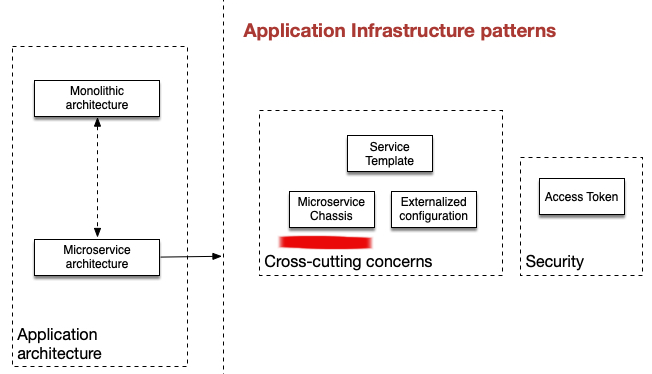
\includegraphics[width=0.5\linewidth]{Images/chassis}
\label{fig:chassis}
\caption{Source: microservices.io}
\end{figure}


\end{frame}

\begin{frame}{Microservice Chassis en Java}
Panorama de chassis en Java
\begin{itemize}
\item DIY
\begin{itemize}
\item Javalin
\item Spark
\item Helidon SE
\end{itemize}
\item Microframework runtimes
\begin{itemize}
\item Apache TomEE
\item Dropwizard
\item Payara Micro
\end{itemize}
\item Full fledged runtimes (ecosistemas)
\begin{itemize}
\item Spring Boot
\item Kumuluz EE
\item Quarkus
\end{itemize}
\end{itemize}


\end{frame}

\begin{frame}{Microservice Chassis}
\textbf{Microservicios en el mundo real}
\begin{itemize}
\item Tu código
\item Chassis
\item Extensiones chassis
\item Bibliotecas independientes
\item Bibliotecas no funcionales -e.g. SCM, Testing-
\item Descriptores para orquestación (Docker, Compose, K8S)
\end{itemize}

\end{frame}


{
    \usebackgroundtemplate{
\includegraphics[width=\paperwidth]{Images/separador}}
    \setbeamercolor{normal text}{fg=white}
    \setbeamercolor{frametitle}{fg=red}
    \usebeamercolor[fg]{normal text}
    \section{Bootstraping microservices}
}


\begin{frame}{Microservice Chassis bootstrap}
La forma Nabenik de iniciar proyectos
\begin{itemize}
\item Nabenik es una empresa que utiliza Java en casi todos sus proyectos y todos los desarrolladores están entrenados en Java EE
\item Apps creciendo desde 2014 -e.g. ERP, POS con geofence-
\item Estudio de desarrollo
\item Necesitabamos mantener un set de dependencias que todos los desarrolladores conozcan
\end{itemize}
\end{frame}

\begin{frame}{Microservice Chassis bootstrap}
Un microservicio típico
\begin{itemize}
\item Lenguaje: Java 11 y a veces Kotlin
\item Java EE / Jakarta EE (Wildfly, Payara, WebLogic)
\item MicroProfile
\item Persistencia: JPA + DeltaSpike Data + persistence.xml + JTA Data source
\item Logs: SLF4J y proveedor CDI
\item Despliegue: Docker + Kubernetes con Eclipse JKube y descriptores YAML
\item Testing: Arquillian, JUnit
\end{itemize}
\end{frame}


\begin{frame}{Microservice Chassis starters}
Nuestra jornada para arrancar microservicios/servicios ligeros
\begin{enumerate}
\item pom.xml personalizado basado en la experiencia (EL POM de referencia)
\item Starters con manual de uso y documentación de extensiones 
\item Proyecto de ejemplo que todo mundo clona y modifica
\item Arquetipo
\end{enumerate}
\end{frame}

\begin{frame}{EL POM de referencia}


\begin{columns}[T] % contents are top vertically aligned
\begin{column}[T]{4cm} % each column can also be its own environment
        \begin{itemize}
            \item Heredado de nuestros proyectos con EAR
            \item Bueno para centralizar versiones
           \item Difícil de mantener sin quebrar algún modulo existente
        \end{itemize}
\end{column}
\begin{column}[T]{10cm} % alternative top-align that's better for graphics

\begin{figure}
        \centering
        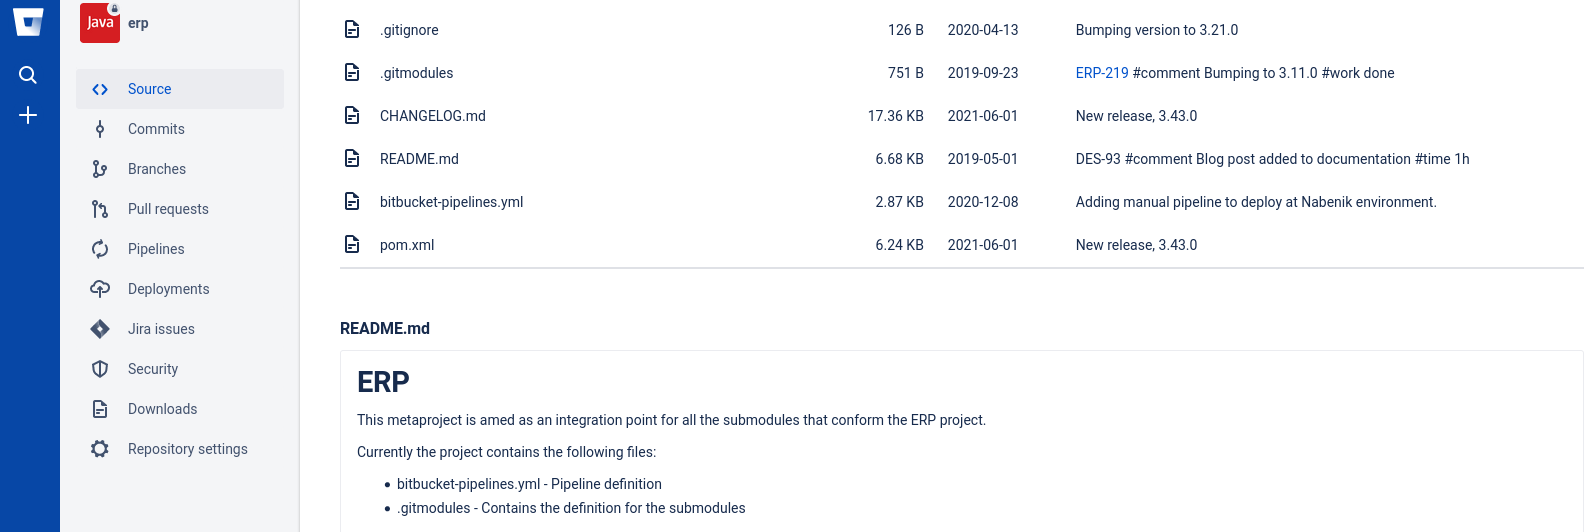
\includegraphics[width=\linewidth]{Images/thepom.png}
        \label{fig:pom}
    \end{figure}
\end{column}
\end{columns}

\end{frame}

\begin{frame}{Starters}

\begin{columns}[T] % contents are top vertically aligned
\begin{column}[T]{4cm} % each column can also be its own environment
        \begin{itemize}
            \item Geniales para principiantes
           \item Iniciar el proyecto y leer la documentación
           \item No siempre un starter incluye una dependencia que te gusta
        \end{itemize}
\end{column}
\begin{column}[T]{10cm} % alternative top-align that's better for graphics

\begin{figure}
        \centering
        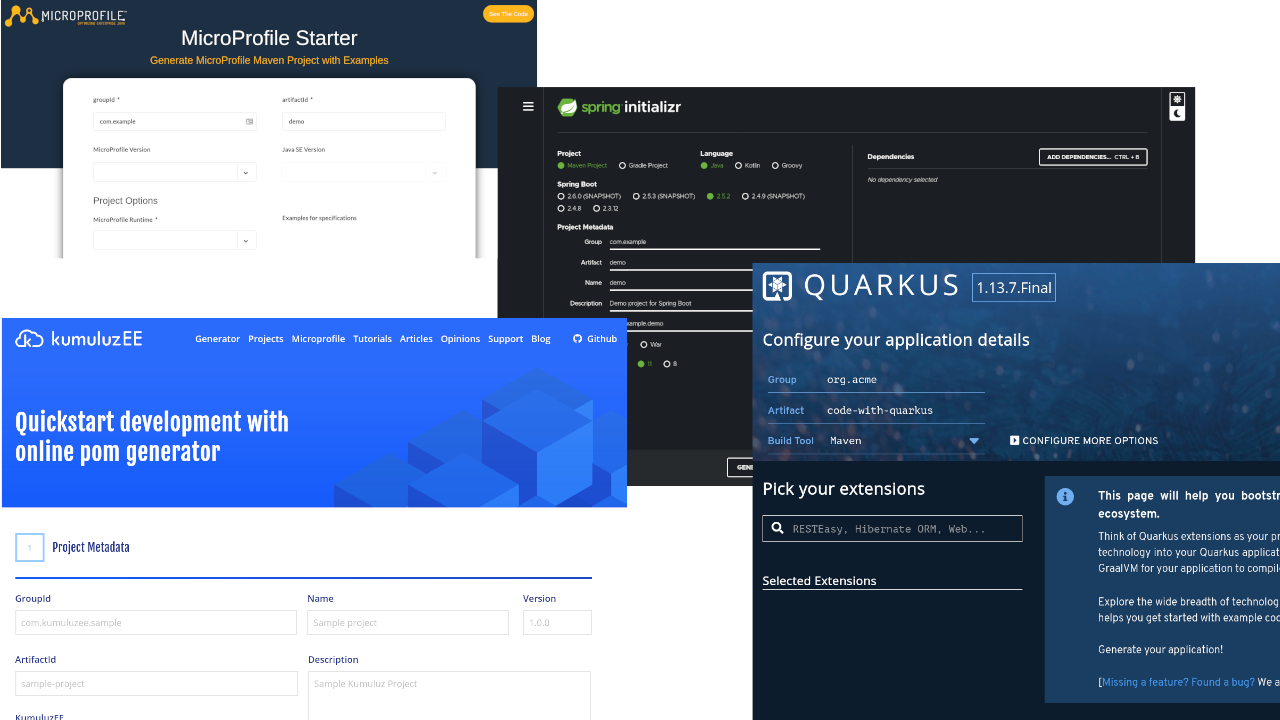
\includegraphics[width=\linewidth]{Images/starters.png}
        \label{fig:starters}
    \end{figure}
\end{column}
\end{columns}
\end{frame}

\begin{frame}{Proyecto de ejemplo}

\begin{columns}[T] % contents are top vertically aligned
\begin{column}[T]{4cm} % each column can also be its own environment
        \begin{itemize}
           \item \textit{Ajustado} a nuestra necesidad
           \item Reemplazamos manualmente package name, app name y versión
           \item Difícil de subir dependencias sin probar apropiadamente
        \end{itemize}
\end{column}
\begin{column}[T]{10cm} % alternative top-align that's better for graphics

\begin{figure}
        \centering
        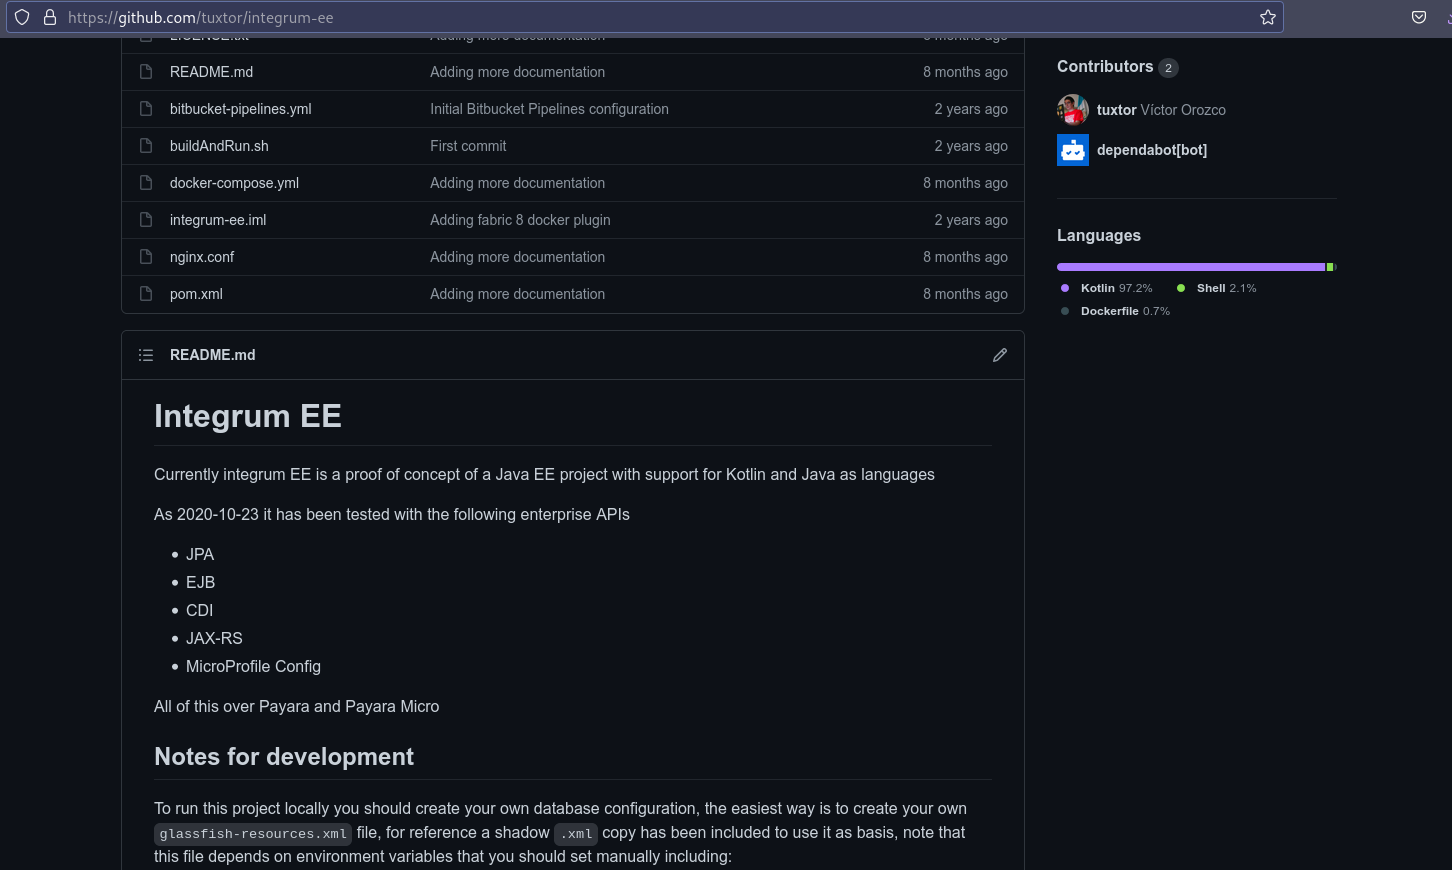
\includegraphics[width=0.9\linewidth]{Images/integrum.png}
        \label{fig:integrum}
    \end{figure}
\end{column}
\end{columns}

\end{frame}

\begin{frame}{Arquetipo}

\begin{columns}[T] % contents are top vertically aligned
\begin{column}[T]{4cm} % each column can also be its own environment
        \begin{itemize}
           \item Basado en el proyecto de ejemplo
           \item Disponible en repositorio interno (y/o Maven Central)
           \item Conjunto de dependencias y runtime aprobado
           \item \textit{Ajustado} desde el día 0
        \end{itemize}
\end{column}
\begin{column}[T]{10cm} % alternative top-align that's better for graphics

\begin{figure}
        \centering
        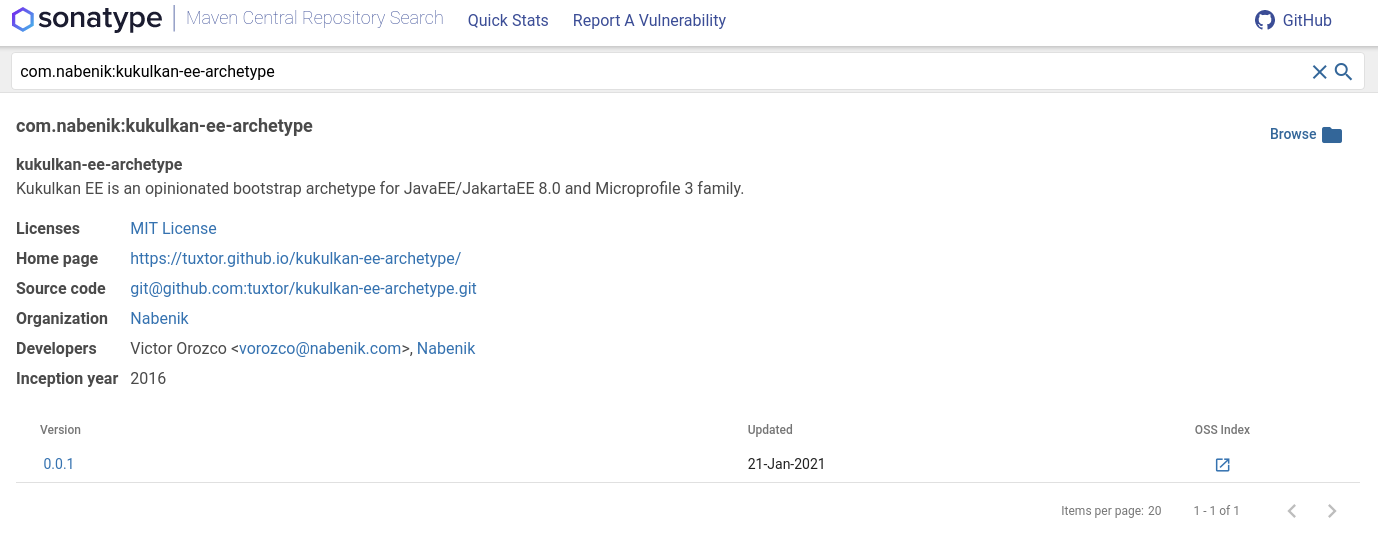
\includegraphics[width=\linewidth]{Images/kukulkan.png}
        \label{fig:archetype}
    \end{figure}
\end{column}
\end{columns}

\end{frame}


{
    \usebackgroundtemplate{
\includegraphics[width=\paperwidth]{Images/separador}}
    \setbeamercolor{normal text}{fg=white}
    \setbeamercolor{frametitle}{fg=red}
    \usebeamercolor[fg]{normal text}
    \section{Creando un arquetipo de microservicio}
}


\begin{frame}{Demo}

        \begin{enumerate}
           \item Crear un proyecto base
           \item Usar el arquetipo maven \textbf{create-from-project}
           \item Reemplazar strings con templates -e.g. Package name, app name, variable-
           \item non-maven resources = ajuste manual
           \item Probar el arquetipo
           \item Subirlo a un repositorio (por si sola es otra presentación)
        \end{enumerate}

\end{frame}

\begin{frame}{Víctor Orozco}
\begin{columns}[T] % contents are top vertically aligned

	\begin{column}[T]{4cm} % alternative top-align that's better for graphics
		\begin{figure}
			\centering
			
\includegraphics[width=\linewidth]{Images/logos}
		\end{figure}
	\end{column}
	\begin{column}[T]{6cm} % each column can also be its own environment
		\begin{itemize}
			\item vorozco@nabenik.com
			\item \href{https://twitter.com/tuxtor}{@tuxtor}
			\item \href{https://vorozco.com}{https://vorozco.com}
			\item \href{https://tuxtor.shekalug.org}{https://tuxtor.shekalug.org}
		\end{itemize}
		\begin{center}
			
\includegraphics[width=0.1\linewidth]{Images/cclogo}
			\\
			This work is licensed under Creative Commons Attribution-NonCommercial-ShareAlike 3.0 Guatemala (CC BY-NC-SA 3.0 GT).
		\end{center}
	\end{column}
\end{columns}
\end{frame}


\end{document}

